%%%%%%%%%%%%%%%%%%%%%%%%%%%%%%%%%%%%%%%%%%%%%%%%%%%%%%%%%%%%%%%%%%%%%%%%%%%%%%%
% Titel:   Pflichtenheft
% Autor:   Nicola K�ser
% Datum:   28.10.2013
% Version: 0.1.0
%%%%%%%%%%%%%%%%%%%%%%%%%%%%%%%%%%%%%%%%%%%%%%%%%%%%%%%%%%%%%%%%%%%%%%%%%%%%%%%
% Versionshinweise und �nderungsprotokol:
%
%  v0.0.1  2013-10-14  Erste Formulierung in Microsoft Word, mit Konzentration
%                      auf den Inhalt, da das Dokument so bald wie m�glich in
%                      LaTeX umformatiert wird.
%  v0.0.2  2013-10-23  Inhalterweiterung
%  v0.1.0  2013-10-28  Konvertierung in LaTeX
%%%%%%%%%%%%%%%%%%%%%%%%%%%%%%%%%%%%%%%%%%%%%%%%%%%%%%%%%%%%%%%%%%%%%%%%%%%%%%%
\documentclass[version=last,fleqn,pointlessnumbers]{scrreprt}
        % first: Ergebniss Kompatibel zu ersten Version; last: Ergebniss entspricht den aktuellen Paketen; fleqn: Formeln linksb�ndig; pointlessnumbers: Kapitelnummerierung ohne Punkt; twoside: Doppelseitiger Druck

% Dokumentangaben
\newcommand{\Titel}{Eurobot 2014 Naherkennung}
\newcommand{\Uebertitel}{Projektarbeit 1 - Dokumentation}
\newcommand{\AutorA}{Nicola K\"aser}
\newcommand{\Dozent}{M. Kucera}
\newcommand{\Datum}{\today}
\newcommand{\Ort}{Burgdorf}
\newcommand{\Version}{0.1.0}



%%%%%%%%%%%%%%%%%%%%%%%%%%%%%%%%%%%%%%%%%%%%%%%%%%%%%%%%%%%%%%%%%%%%%%%%%%%%%%%
% Pakete
%%%%%%%%%%%%%%%%%%%%%%%%%%%%%%%%%%%%%%%%%%%%%%%%%%%%%%%%%%%%%%%%%%%%%%%%%%%%%%%
%%%%%%%%%%%%%%%%%%%%%%%%%%%%%%%%%%%%%%%%%%%%%%%%%%%%%%%%%%%%%%%%%%%%%%%%%%%%%%%
% Titel:   Bericht - Pakete
% Autor: Simon Grossenbacher  
% Datum:   27.09.2013
% Version: 1.0.0
%%%%%%%%%%%%%%%%%%%%%%%%%%%%%%%%%%%%%%%%%%%%%%%%%%%%%%%%%%%%%%%%%%%%%%%%%%%%%%%
%
%:::Change-Log:::
% Versionierung erfolgt auf folgende Gegebenheiten: -1. Release Versionen
%                                                   -2. Neue Kapitel
%                                                   -3. Fehlerkorrekturen
%
% 0.0.0       Erstellung der Datei
%
%:::Hinweis:::
% Indexerstellung: makeindex -s report.ist report.idx
%   Umlaute m�ssen separat behandelt werden!
%%%%%%%%%%%%%%%%%%%%%%%%%%%%%%%%%%%%%%%%%%%%%%%%%%%%%%%%%%%%%%%%%%%%%%%%%%%%%%%

%Sprach-Optionen
\usepackage[ngerman]{babel} %neue deutsche Rechtschreibung
\usepackage[T1]{fontenc}  %richtige Worttrennung
%\usepackage[applemac]{inputenc}                % Mac - load extended character set (ISO 8859-1)
%\usepackage[latin1]{inputenc}                   % Unix/Linux - load extended character set (ISO 8859-1)
\usepackage[ansinew]{inputenc}                 % Windows - load extended character set (ISO 8859-1)
%\usepackage[utf8]{inputenc}                    % UTF-8 encoding

%Zeilenabstand
\usepackage{setspace}

%Mehr Tabellenoptionen
\usepackage{tabularx}
\usepackage{longtable}

%Listen
\usepackage{enumitem}

%Besserer Flattersatz
\usepackage{ragged2e}

%Gleiten verhindern
\usepackage{float}
\usepackage{placeins}

%Z�hler per Seite resetten (z.B. Fussnoten-Index)
\usepackage{perpage}

%Ueberschriften anpassen
\usepackage{titlesec} 

%Farben
\usepackage{color}
\usepackage{colortbl} %F�r farbige Tabellen

%PDF zu Dokument hinzufuegen
\usepackage[final]{pdfpages}

%Grafiken verwalten
\usepackage{graphicx}
\usepackage[absolute]{textpos}

%Zeichnen
%\usepackage{pst-pdf}
%\usepackage{pst-all}

%Listnings verwalten
\usepackage{listings}

%Kopf- Fusszeile (Optionen m�ssen direkt �bergeben werden)
\usepackage[automark, %Automatisches aktualisieren der Chapter-Titel
%            headsepline,  %Linie Kopfzeile
%            footsepline,  %Linie fusszeilezeile
%            markuppercase,
            plainfootsepline  %Plain-Style auch mit Linie versehen
            ]{scrpage2}

%Flexible Argumente bei Funktionen
\usepackage{xargs}

%erweiterte Steuerfunktionen
\usepackage{ifthen}

%Index f�r Stichwortverzeichnis
\usepackage{makeidx}

%Index f�r Literaturverzeichnis
\usepackage[babel,german=quotes]{csquotes}
%\usepackage[backend=biber,style=numeric,defernumbers=true,sorting=nyt]{biblatex}
\usepackage[backend=bibtex,defernumbers=true]{biblatex}
\bibliography{bibliography}
\defbibheading{lit}{\section{Literatur}}
\defbibheading{pic}{\section{Abbildungen}}

%Zusaetzliche Symbole direkt im Text
\usepackage{textcomp}
\usepackage{amssymb}

%Einheit kontrolliert eingeben
\usepackage{units}

%dynamische Datumsausgabe
\usepackage[german]{isodate}

%Zusaetzlich Mathemtiksymbole
\usepackage{amsmath}
\usepackage{mathtools}

%Besser Handling von internen Countern und Berechnungen
\usepackage{calc}

%TODOs anbringen am Rand
\usepackage{todonotes}

%Hyperlinks (Muss das letzte geladene Paket sein)
\usepackage[bookmarks=true, %Verzeichnis generieren
            bookmarksopen=true, %Verzeichnis �ffnen
            bookmarksopenlevel=\tocmaxdepth, %Tiefe der Verzeichnis�ffnung
            unicode=false, %non-Latin Zeichen
            pdftoolbar=true, %PDF-Viewer Toolbar
            pdfmenubar=true, %PDF-Viewer Men�?
            pdffitwindow=true, %Fenster an Seite anpassen beim �ffnen
            pdftitle={\Titel}, %Titel
            %pdfauthor={\Autor1, \Autor2, \Autor3}, %Autor
            pdfsubject={\Uebertitel}, %Thema
%            pdfcreator={\Autor1, \Autor2, \Autor3}, %Ersteller des Dokuments
%            pdfproducer={\Autor1, \Autor2 \Autor3}, %Produzent des Dokuments
            pdfnewwindow=true, %Links in neuem Fenster
            colorlinks=true, %false: Boxen-Links; true: Farben-Links
            linkcolor=black, %Farbe von internen Links
            citecolor=black, %Farbe von Links zu Bibliography
            filecolor=magenta, %Farbe von Links zu Dateien
            urlcolor=blue %Farbe von externen Links
            ]{hyperref}
            
%Glossar/Abk�rzungsverzeichnis
\usepackage[acronym,makeindex]{glossaries}




%%%%%%%%%%%%%%%%%%%%%%%%%%%%%%%%%%%%%%%%%%%%%%%%%%%%%%%%%%%%%%%%%%%%%%%%%%%%%%%
% Funktionen
%%%%%%%%%%%%%%%%%%%%%%%%%%%%%%%%%%%%%%%%%%%%%%%%%%%%%%%%%%%%%%%%%%%%%%%%%%%%%%%
%%%%%%%%%%%%%%%%%%%%%%%%%%%%%%%%%%%%%%%%%%%%%%%%%%%%%%%%%%%%%%%%%%%%%%%%%%%%%%%
% Titel:   Bericht - Funktionen
% Autor:   Simon Grossenbacher
%          Nicola K�ser (v1.1.0)
% Datum:   27.09.2013
% Version: 1.1.0
%%%%%%%%%%%%%%%%%%%%%%%%%%%%%%%%%%%%%%%%%%%%%%%%%%%%%%%%%%%%%%%%%%%%%%%%%%%%%%%
%
%:::Change-Log:::
% Versionierung erfolgt auf folgende Gegebenheiten: -1. Release Versionen
%                                                   -2. Neue Kapitel
%                                                   -3. Fehlerkorrekturen
%
% 0.0.0       Erstellung der Datei
% 1.0.0       Release
% 1.1.0       Erg�nzungen
%
%:::Hinweis:::
% Indexerstellung: makeindex -s report.ist report.idx
%   Umlaute m�ssen separat behandelt werden!
%%%%%%%%%%%%%%%%%%%%%%%%%%%%%%%%%%%%%%%%%%%%%%%%%%%%%%%%%%%%%%%%%%%%%%%%%%%%%%%

%%%%%%%%%%%%%%%%%%%%%%%%%%%%%%%%%%%%%%%%%%%%%%%%%%%%%%%%%%%%%%%%%%%%%%%%%%%%%%%
% Text tiefstellen
% param #1 Text
%%%%%%%%%%%%%%%%%%%%%%%%%%%%%%%%%%%%%%%%%%%%%%%%%%%%%%%%%%%%%%%%%%%%%%%%%%%%%%%
\newcommand{\low}[1]{\textsubscript{#1}}



%%%%%%%%%%%%%%%%%%%%%%%%%%%%%%%%%%%%%%%%%%%%%%%%%%%%%%%%%%%%%%%%%%%%%%%%%%%%%%%
% Text hochstellen
% param #1 Text
%%%%%%%%%%%%%%%%%%%%%%%%%%%%%%%%%%%%%%%%%%%%%%%%%%%%%%%%%%%%%%%%%%%%%%%%%%%%%%%
\newcommand{\high}[1]{\textsuperscript{#1}}



%%%%%%%%%%%%%%%%%%%%%%%%%%%%%%%%%%%%%%%%%%%%%%%%%%%%%%%%%%%%%%%%%%%%%%%%%%%%%%%
% Schrift anpassen
% param #1 Schriftfamilie: ptm Times
%                          phv Helvetica
%                          pcr Courier
%                          pbk Bookman
%                          pag Avant Garde
%                          ppl Palatino
%                          pch Charter
%                          pnc New Century Schoolbook
%                          put Utopia
% param #2 Strichdicke/Zeichenbreite: b  bold
%                                     m  medium
% param #3 Schriftform: n   normal
%                       it  italic
%                       sl  slanted
%                       sc  small caps
%                       ui  upright italic
% note {\changefont{#1}{#2}{#3} Hallo Welt} Teilbereich aendern
%%%%%%%%%%%%%%%%%%%%%%%%%%%%%%%%%%%%%%%%%%%%%%%%%%%%%%%%%%%%%%%%%%%%%%%%%%%%%%%
\newcommand{\changefont}[3]{\fontfamily{#1} \fontseries{#2} \fontshape{#3} \selectfont}



%%%%%%%%%%%%%%%%%%%%%%%%%%%%%%%%%%%%%%%%%%%%%%%%%%%%%%%%%%%%%%%%%%%%%%%%%%%%%%%
% Zum Beispiel abkuerzen ohne Trennung
% param none
%%%%%%%%%%%%%%%%%%%%%%%%%%%%%%%%%%%%%%%%%%%%%%%%%%%%%%%%%%%%%%%%%%%%%%%%%%%%%%%
\newcommand{\zB}{z.~B.}



%%%%%%%%%%%%%%%%%%%%%%%%%%%%%%%%%%%%%%%%%%%%%%%%%%%%%%%%%%%%%%%%%%%%%%%%%%%%%%%
% Formeleintrag
% param #1 Formel
% param #2 Parameter Beschreibung im Tabellensyntax
% param #3 Formel-Label (optional)
%%%%%%%%%%%%%%%%%%%%%%%%%%%%%%%%%%%%%%%%%%%%%%%%%%%%%%%%%%%%%%%%%%%%%%%%%%%%%%%
%Savebox fuer Parameterbeschreibung
\newsavebox{\myendhook}  % for the tabulars
\makeatletter
\def\tagform@#1{{(\maketag@@@{\ignorespaces#1\unskip\@@italiccorr)}
\makebox[0pt][r]{% after the equation number
\makebox[0.5\textwidth][l]{\usebox{\myendhook}}%
}%
\global\sbox{\myendhook}{}% clear box content
}}
\makeatother
%Kommando definieren
\newcommandx{\formula}[3][3=\empty,usedefault]{
	\sbox{\myendhook}{%
		\begin{footnotesize}%
			\begin{tabular}{>{$}l<{$} >{\RaggedRight}p{.33\textwidth}}%0.33 \begin{tabular}{@{}l >{\RaggedRight}p{.33\textwidth}}
				#2%\ifthenelse{\equal{#2}{\empty}}{ }{#2}
			\end{tabular}
		\end{footnotesize}}
	%
	\begin{equation}
		\ifthenelse{\equal{#3}{\empty}}
		{}
		{\label{#3}}%anstatt equation
		\boxed{\begin{split}#1\end{split}}
		%\begin{split}#1\end{split}
	\end{equation}  %anstatt equation
}



%%%%%%%%%%%%%%%%%%%%%%%%%%%%%%%%%%%%%%%%%%%%%%%%%%%%%%%%%%%%%%%%%%%%%%%%%%%%%%%
% Bildereintrag
% param #1 Pfad zum Bild
% param #2 Groesse: z.B. scale=0.5
% param #3 Bildunterschrift (optional)
% param #4 Bildunterschrift im Abbildungsverzeichnis (optional)
% param #5 Bildlabel (optional)
%%%%%%%%%%%%%%%%%%%%%%%%%%%%%%%%%%%%%%%%%%%%%%%%%%%%%%%%%%%%%%%%%%%%%%%%%%%%%%%
\newlength{\imagewidth}
\newlength{\imageheight}
\newcommandx{\image}[5][3=\empty,4=\empty:,5=\empty,usedefault]{
	\begin{figure}[H]%H htbp
		\centering
		\settowidth{\imagewidth}{\includegraphics[#2]{#1}}
		\settoheight{\imageheight}{\includegraphics[#2]{#1}}
		\ifdim\imagewidth<\textwidth
			\ifdim\imageheight<\textheight
				\includegraphics[#2]{#1}
			\else
				\includegraphics[height=\textheight]{#1}
			\fi
		\else
			\ifdim\imageheight<\textheight
				\includegraphics[width=\textwidth]{#1}
			\else
				\setlength{\imageheight}{\imageheight-\textheight}
				\setlength{\imagewidth}{\imagewidth-\textwidth}
				\ifdim\imageheight<\imagewidth
					\includegraphics[width=\textwidth]{#1}
				\else
					\includegraphics[height=\textheight]{#1}
				\fi
			\fi
		\fi
		\ifthenelse{\equal{#5}{\empty}}
		{
			\ifthenelse{\equal{#3}{\empty}}{}{\caption{#3}}
			\ifthenelse{\equal{#4}{\empty}}{}{\label{#4}}
		}
		{
			\caption[#4]{#3}
			\label{#5}
		}
	\end{figure}
}



%%%%%%%%%%%%%%%%%%%%%%%%%%%%%%%%%%%%%%%%%%%%%%%%%%%%%%%%%%%%%%%%%%%%%%%%%%%%%%%
% Bildereintrag fuer Tabellen
% param #1 Pfad zum Bild
% param #2 Groesse: z.B. scale=0.5
%%%%%%%%%%%%%%%%%%%%%%%%%%%%%%%%%%%%%%%%%%%%%%%%%%%%%%%%%%%%%%%%%%%%%%%%%%%%%%%
\newlength{\myx}  % Variable zum Speichern der Bildbreite
\newlength{\myy}  % Variable zum Speichern der Bildh�he
\newcommand{\imagetotab}[2][\relax]{%
% Abspeichern der Bildabmessungen
\settowidth{\myx}{\includegraphics[{#1}]{#2}}%
\settoheight{\myy}{\includegraphics[{#1}]{#2}}%
% das eigentliche Einf�gen
\parbox[c][1.1\myy][c]{\myx}{%
\includegraphics[{#1}]{#2}}%
}



%%%%%%%%%%%%%%%%%%%%%%%%%%%%%%%%%%%%%%%%%%%%%%%%%%%%%%%%%%%%%%%%%%%%%%%%%%%%%%%
% Kapitel ohne Nummerierung aber mit Angabe im Inhaltsverzeichnis
% param #1 Kapitelname
%%%%%%%%%%%%%%%%%%%%%%%%%%%%%%%%%%%%%%%%%%%%%%%%%%%%%%%%%%%%%%%%%%%%%%%%%%%%%%%
\newcommand{\chapternn}[1]{\chapter*{#1} \addcontentsline{toc}{chapter}{#1}}




%%%%%%%%%%%%%%%%%%%%%%%%%%%%%%%%%%%%%%%%%%%%%%%%%%%%%%%%%%%%%%%%%%%%%%%%%%%%%%%
% Redefinition von \cite, sodass bei jedem Aufruf ein Z�hler inkrementiert
% wird. Dieser kann verwendet werden, damit das Quellenkapitel nur bei der
% Verwendung von \cite eingef�gt wird (\ifnum\value{numcite}>0 ... \fi).
%%%%%%%%%%%%%%%%%%%%%%%%%%%%%%%%%%%%%%%%%%%%%%%%%%%%%%%%%%%%%%%%%%%%%%%%%%%%%%%
% Neuer Z�hler f�r \cite
\newcounter{numcite}
% \cite als \oldcite speichern
\let\oldcite\cite
% \cite neu definieren, sodass Z�hler jedesmal inkrementiert wird
\renewcommand\cite[1]{\oldcite{#1} \stepcounter{numcite}}
%
% Neuer Z�hler f�r \cite
\newcounter{citenum}
% \cite als \oldcite speichern
\let\oldcite\cite
% \cite neu definieren, dass Z�hler jedesmal inkrementiert wird
\renewcommand\cite[1]{\oldcite{#1}\stepcounter{citenum}}
% Optionale Definition, damit Abbildungsverzeichnis und Tabellenverzeichnis auf gleicher Seite
\newcommand{\listsOnSamePage}{}


%%%%%%%%%%%%%%%%%%%%%%%%%%%%%%%%%%%%%%%%%%%%%%%%%%%%%%%%%%%%%%%%%%%%%%%%%%%%%%%
% Farben
%%%%%%%%%%%%%%%%%%%%%%%%%%%%%%%%%%%%%%%%%%%%%%%%%%%%%%%%%%%%%%%%%%%%%%%%%%%%%%%
\RequirePackage{color}                          % Color (not xcolor!)
% Allgemein
\definecolor{grey}{gray}{0.7}
\definecolor{lightgrey}{gray}{0.9}

% BFH
\definecolor{bfhred}{rgb}{0.776,0,0.066}
\definecolor{brickred}{cmyk}{0,0.89,0.94,0.28}      % Brickred
\definecolor{bfhblue}{rgb}{0.396,0.49,0.56}         % Blue
\definecolor{bfhorange}{rgb}{0.961,0.753,0.196}     % Orange
\definecolor{bfhorangelight}{RGB}{246,216,136}      % Orange Light

% Listing
\definecolor{hellgelb}{rgb}{1,1,0.8}
\definecolor{listingbackground}{RGB}{246,216,136} 
\definecolor{colKeys}{rgb}{0,0,1}
\definecolor{colIdentifier}{rgb}{0,0,0}
\definecolor{colComments}{rgb}{0.2,0.8.3}
\definecolor{colString}{rgb}{0,0.5,0}

% Tabellen
%\rowcolors{1}{bfhblue}{bfhorangelight}


%%%%%%%%%%%%%%%%%%%%%%%%%%%%%%%%%%%%%%%%%%%%%%%%%%%%%%%%%%%%%%%%%%%%%%%%%%%%%%%
% Schrift
%%%%%%%%%%%%%%%%%%%%%%%%%%%%%%%%%%%%%%%%%%%%%%%%%%%%%%%%%%%%%%%%%%%%%%%%%%%%%%%
% Standardschriftgr�sse
\KOMAoptions{fontsize=11pt}

% Zeilenabstand
%\onehalfspacing  % 1.5 Zeilenabstand

% Schrift eines bestimmten Elements anpassen/erstellen z.B. captionlabel
%\setkomafont{captionlabel}{\itshape}  % definert Schriftart f�r captionlabel
%\addkomafont{captionlabel}{\itshape}  % f�gt Eigenschaft zu captionlabel hinzu

% Formatvorlage anpassen
\setkomafont{pageheadfoot}{\footnotesize\sffamily}  % Kopf-/Fusszeile \normalfont
\setkomafont{pagenumber}{\normalfont\sffamily\bfseries}  % Seitennummer



%%%%%%%%%%%%%%%%%%%%%%%%%%%%%%%%%%%%%%%%%%%%%%%%%%%%%%%%%%%%%%%%%%%%%%%%%%%%%%%
% Gleitobjekte (Bilder/Tabellen/Formeln)
%%%%%%%%%%%%%%%%%%%%%%%%%%%%%%%%%%%%%%%%%%%%%%%%%%%%%%%%%%%%%%%%%%%%%%%%%%%%%%%
% Formelneinzug = wie Aufz�hlungseinzug
\setlength{\mathindent}{0.6\leftmargini}

% Gleitobjekte
\setlength{\intextsep}{8mm +2mm -2mm}%\intextsep10mm plus3mm minus2mm
%\setlength{\textfloatsep}{100mm plus5pt minus3pt}

% Bild-Tabellen Beschriftung linksb�ndig
%\KOMAoptions{captions=nooneline}  % linksb�ndig
\setcaphanging  % Mehrzeilige Beschriftung erh�lt Einzug



%%%%%%%%%%%%%%%%%%%%%%%%%%%%%%%%%%%%%%%%%%%%%%%%%%%%%%%%%%%%%%%%%%%%%%%%%%%%%%%
% Seiteneinstellungen
%%%%%%%%%%%%%%%%%%%%%%%%%%%%%%%%%%%%%%%%%%%%%%%%%%%%%%%%%%%%%%%%%%%%%%%%%%%%%%%
% Dokumentstadium
\KOMAoptions{draft=false}  % Erleichert das erkennen von Fehlern im Entwurfsstadium

% Papierformat
\KOMAoptions{paper=A4}  % Format (Bei direkten Massangaben: 5cm:3cm)
%\KOMAoptions{paper=landscape}  % Ausrichtung  (Standard Portrait)
\KOMAoptions{pagesize=automedia}  % Angabe f�r Ausgangstreiber

% Bindekorrektur
%\KOMAoptions{BCOR=0.1cm}  % Bindekorrektur (Bereich der durchs Binden verloren geht)

% Gr�sse des Satzspiegels
\KOMAoptions{DIV=11}  % Gr�sse des Satzspiegels (Faktor ab 4), siehe S.38 scrguide.pdf; nur f�r A4 existieren Voreinstellungen, sonst calc o. classic als Option

% Randbereich
\KOMAoptions{mpinclude=false}  % Definiert ob der Randbereich zum Textk�rper hinzugez�hlt werden soll oder nicht -> TRUE nur bei Sonderf�llen

% Doppelspaltiges Dokument
\KOMAoptions{twocolumn=false}

% Absatzabstand
\KOMAoptions{parskip=true}

% Seitenstyle
\pagestyle{scrheadings}  % myheadings scrheadings

% Platzierzung letzte Zeile
\raggedbottom  % Letze Zeile liegt dort wo sie gerade ist -> unterschiedlicher vertikaler Abstand zu Blatt Ende (unerw�nscht bei doppelseitigem Druck)
%\flushbottom  % Letze Zeile immer am Schluss -> evtl. unterschiedliche Absatzabst�nde



%%%%%%%%%%%%%%%%%%%%%%%%%%%%%%%%%%%%%%%%%%%%%%%%%%%%%%%%%%%%%%%%%%%%%%%%%%%%%%%
% Kopf-/Fusszeile
%%%%%%%%%%%%%%%%%%%%%%%%%%%%%%%%%%%%%%%%%%%%%%%%%%%%%%%%%%%%%%%%%%%%%%%%%%%%%%%
% Kopfzeile
%\clearscrheadfoot  % Alle Vorgaben l�schen (plain und scrheadings)
\renewcommand*{\chaptermarkformat}{  % headmark ohne Kapitelnummer
%\chapappifchapterprefix{\ }\thechapter\autodot\enskip
}
% i: Links; c: Zentrum; o:Rechts; [Auf Kapitelstartseiten]; {Auf allen anderen Seiten}
\ihead[]{\textcolor{bfhblue}{\headmark}}  % Chapter Titel in Kopfzeile
\chead[]{}
\ohead[\textcolor{bfhblue}{\Titel, v\Version}]{\textcolor{bfhblue}{\Titel, v\Version}}  % Titel mit Version in Kopfzeile

% Fusszeile
\ifoot[\textcolor{bfhblue}{Berner Fachhochschule}]{\textcolor{bfhblue}{Berner Fachhochschule}}  % plain und scrheadings mit Dokumenttitel versehen
\cfoot[]{}
\ofoot[\textcolor{bfhblue}{\pagemark}]{\textcolor{bfhblue}{\pagemark}}  % plain und scrheadings mit Seitennummer versehen



%%%%%%%%%%%%%%%%%%%%%%%%%%%%%%%%%%%%%%%%%%%%%%%%%%%%%%%%%%%%%%%%%%%%%%%%%%%%%%%
% Fussnote
%%%%%%%%%%%%%%%%%%%%%%%%%%%%%%%%%%%%%%%%%%%%%%%%%%%%%%%%%%%%%%%%%%%%%%%%%%%%%%%
% Fussnote
%\KOMAoptions{footnotes=multiple}  % Fussnotennummern durch "," trennen



% Satzspiegel neu berechnen -> falls andere Schriftengeladen werden und/oder Zeilenabstand ver�ndert wird
\recalctypearea



%%%%%%%%%%%%%%%%%%%%%%%%%%%%%%%%%%%%%%%%%%%%%%%%%%%%%%%%%%%%%%%%%%%%%%%%%%%%%%%
% Paket Listings Konfiguration
%%%%%%%%%%%%%%%%%%%%%%%%%%%%%%%%%%%%%%%%%%%%%%%%%%%%%%%%%%%%%%%%%%%%%%%%%%%%%%%

% XML
\lstdefinestyle{XML}{numbers=left, 
    basicstyle=\scriptsize\ttfamily,
    numberstyle=\tiny, 
    xleftmargin=0.5\leftmargin,
    xrightmargin=\rightmargin,
    numbersep=5pt,
    backgroundcolor=\color{listingbackground}, 
    breaklines=true,
    captionpos=b,
    language=XML}

% MATlAB
\lstdefinestyle{Matlab}{numbers=left, 
    basicstyle=\scriptsize\ttfamily,
    numberstyle=\tiny,
    xleftmargin=0.5\leftmargin,
    xrightmargin=\rightmargin,
    numbersep=5pt,
    backgroundcolor=\color{listingbackground},
    identifierstyle=\color{colIdentifier},
    keywordstyle=\color{colKeys},
    stringstyle=\color{colString},
    commentstyle=\color{colComments},
    breaklines=true,
    captionpos=b,
    language=Matlab}

% ANSI C
\lstdefinestyle{C}{numbers=left, 
    basicstyle=\scriptsize\ttfamily,
    numberstyle=\tiny,
    xleftmargin=0.5\leftmargin,
    xrightmargin=\rightmargin,
    numbersep=5pt,
    backgroundcolor=\color{listingbackground},
    identifierstyle=\color{colIdentifier},
    keywordstyle=\color{colKeys},
    stringstyle=\color{colString},
    commentstyle=\color{colComments},
    breaklines=true,
    captionpos=b,
    language=[ANSI] C}


\makeindex  % Ab hier Indexieren
%%%%%%%%%%%%%%%%%%%%%%%%%%%%%%%%%%%%%%%%%%%%%%%%%%%%%%%%%%%%%%%%%%%%%%%%%%%%%%%
% Dokument Anfang
%%%%%%%%%%%%%%%%%%%%%%%%%%%%%%%%%%%%%%%%%%%%%%%%%%%%%%%%%%%%%%%%%%%%%%%%%%%%%%%
\begin{document}
%
%
%%%%%%%%%%%%%%%%%%%%%%%%%%%%%%%%%%%%%%%%%%%%%%%%%%%%%%%%%%%%%%%%%%%%%%%%%%%%%%%
% Titelseite
%%%%%%%%%%%%%%%%%%%%%%%%%%%%%%%%%%%%%%%%%%%%%%%%%%%%%%%%%%%%%%%%%%%%%%%%%%%%%%%
%%%%%%%%%%%%%%%%%%%%%%%%%%%%%%%%%%%%%%%%%%%%%%%%%%%%%%%%%%%%%%%%%%%%%%%%%%%%%%%
% Titel:   Titelseite
% Autor:   S. Grossenbacher
% Datum:   15.10.2012
% Version: 3.0.0
%%%%%%%%%%%%%%%%%%%%%%%%%%%%%%%%%%%%%%%%%%%%%%%%%%%%%%%%%%%%%%%%%%%%%%%%%%%%%%%
%
%:::Change-Log:::
% Versionierung erfolgt auf folgende Gegebenheiten: -1. Stelle Semester
%                                                   -2. Stelle neuer Inhalt
%                                                   -3. Fehlerkorrekturen
%
% 3.0.0       Erstellung der Datei
%
%%%%%%%%%%%%%%%%%%%%%%%%%%%%%%%%%%%%%%%%%%%%%%%%%%%%%%%%%%%%%%%%%%%%%%%%%%%%%%%
%
%Zeilenabstand wider auf normalen Wert zur�ckstellen
\begin{spacing}{1}
    %
    %Titelseiteumgebung f�r eigene Kreation, sonst \maketitle
    \begin{titlepage}   
        \newlength{\unitlengthtmp}
        \setlength{\unitlengthtmp}{\unitlength}
        \setlength{\unitlength}{1mm}   
        \setlength{\TPHorizModule}{\textwidth}
        \setlength{\TPVertModule}{\textheight} 
        %
        % BFH Logo
        
\includegraphics[scale=1.25]{titlepage/image/bfh_logo}\todo{Technik und Informatik}
        %
        % Linien
        \begin{textblock}{1}[0,0](0,0)
	        \begin{picture}(0,130)
	            \put(28.5,0){\color{bfhblue}\rule{\textwidth}{1.2mm}}
		        \put(28.5,40){\color{bfhblue}\rule{\textwidth}{1.2mm}}		
	        \end{picture}
        \end{textblock} 
        %
        %Zentrierte Titel
        \begin{flushleft}
            \vspace*{4.08cm}
            \textsf{\textbf{\noindent{\Huge{\textcolor{bfhblue}{\Titel}}}}}\\[0.4cm]
            \textsf{\huge{\textcolor{bfhblue}{\Uebertitel}}}
            %
            %Angaben zum Dokument
            \begin{vfill}
                \begin{tabularx}{\textwidth}{lX}
                    \textsf{Autor} %& \textsf\AutorA\\
                                   %& \textsf\AutorB\\
                                   %& \textsf\AutorC\vspace{5pt}\\
                                   & \textsf\AutorA\vspace{5pt}\\
                    \textsf{Dozent} & \textsf\Dozent\vspace{5pt}\\
                    \textsf{Datum} & \textsf\Datum\\
                    \textsf{Ort} & \textsf\Ort\vspace{5pt}\\
                    \textsf{Version} & \textsf\Version\\ 
                    &\\
                    &\\
                    &\\
                    \multicolumn{2}{p{\textwidth-2\tabcolsep}}{\textsf{%%%%%%%%%%%%%%%%%%%%%%%%%%%%%%%%%%%%%%%%%%%%%%%%%%%%%%%%%%%%%%%%%%%%%%%%%%%%%%%
% Titel:   Titeltext
% Autor:   Nicola K�ser
%%%%%%%%%%%%%%%%%%%%%%%%%%%%%%%%%%%%%%%%%%%%%%%%%%%%%%%%%%%%%%%%%%%%%%%%%%%%%%%

In einem abteilungs\"ubergreifenden Team nimmt die Berner Fachhochschule beim allj\"ahrlich durchgef\"uhrten Eurobot Robotik-Wettbewerb teil. Ein wichtiger Punkt bei einem solchen Projekt ist immer auch die Sicherheit des Roboters. Aus diesem Grund muss die n\"ahere Umgebung um den Roboter fortlaufend \"uberwacht werden. So k\"onnen Zusammenst\"osse mit anderen Robotern und/oder anderen Objekten verhindert werden. Dieses Dokument beschreibt die Bearbeitung dieser Teilaufgabe.}}\\
                \end{tabularx}
            \end{vfill}
        \end{flushleft}
        \setlength{\unitlength}{\unitlengthtmp}
    \end{titlepage}
\end{spacing}


\thispagestyle{empty}
\cleardoublepage  % Leere Seite nach Titelseite einf�gen
%
%
%
\pagenumbering{roman}  % R�misch Nummerieren ab hier
%
%
%
%%%%%%%%%%%%%%%%%%%%%%%%%%%%%%%%%%%%%%%%%%%%%%%%%%%%%%%%%%%%%%%%%%%%%%%%%%%%%%%
% Abstract + Selbstaendige Arbeit
%%%%%%%%%%%%%%%%%%%%%%%%%%%%%%%%%%%%%%%%%%%%%%%%%%%%%%%%%%%%%%%%%%%%%%%%%%%%%%%
%%%%%%%%%%%%%%%%%%%%%%%%%%%%%%%%%%%%%%%%%%%%%%%%%%%%%%%%%%%%%%%%%%%%%%%%%%%%%%%
% Titel:   Abstract
% Autor:   Nicola K�ser
%%%%%%%%%%%%%%%%%%%%%%%%%%%%%%%%%%%%%%%%%%%%%%%%%%%%%%%%%%%%%%%%%%%%%%%%%%%%%%%

%%%%%%%%%%%%%%%%%%%%%%%%%%%%%%%%%%%%%%%%%%%%%%%%%%%%%%%%%%%%%%%%%%%%%%%%%%%%%%%
\chapter*{Abstract}
In einem abteilungs�bergreifenden Team nimmt die Berner Fachhochschule bei einem allj�hrlich durchgef�hrten Robotik-Wettbewerb namens Eurobot teil. In diesem Wettbewerb k�nnen sich Studenten aus unterschiedlichen Schulen in der Entwicklung eines autonomen Roboters messen. Die Anforderungen an die Roboter werden von den Organisatoren jedes Jahr neu aufgestellt und unter einer zusammenfassenden Thematik ver�ffentlicht. F�r das Jahr 2014 sind zwei Roboter unterschiedlicher Gr�sse erlaubt. Das Thema lautet "`PrehistoBot"' und beinhaltet folgende Aufgaben:
%
\begin{description}[leftmargin=!,labelwidth=\widthof{\bfseries Mammuts:},noitemsep]
	\item[Mammuts:] Mammutfiguren an den Spielfeldseiten mit Klebeb�llen und Netz bewerfen
	\item[Freskos:] Zeichnungen an Spielfeldwand anbringen
	\item[Fr�chte:] Fr�chte von B�umen an Spielfeldrand pfl�cken
	\item[Feuer:] Spielkl�tze im Spielfeld sammeln und korrekt platzieren
\end{description}
%
Damit die Roboter die Aufgaben ohne Zusammenst�sse diese Aufgaben erledigen kann, m�ssen sie �ber ein System verf�gen, womit sie die n�here Umgebung um sich fortlaufend �berwachen k�nnen.
\par Daher stellte ich mir die Aufgabe, ein solches System zu entwickeln und teilte es in folgende Teilaufgaben: Recherche nach geeigneten Sensoren, Evaluation ausgew�hlter Sensoren, Entscheidung und Realisation.
\par Ich kam zum Schluss, dass die Verwendung von zwei Sensortypen, basierend auf Infrarot sowie Ultraschall, die Zuverl�ssigkeit des Systems am Besten gew�hrleistet. Das Ergebnis der Arbeit ist die Hard- und Software f�r die Naherkennung.
\todo{Evtl. offene Fragen} % Z.B.: Noch offen ist die Art Informations�bergabe an das Kernteam, da f�r beide Roboter eine unterschiedliche...
\chapter*{Selbst�ndige Arbeit}
\label{ch:Selbst�ndige Arbeit}
Ich erkl�re ausdr�ckich, dass es sich bei dieser von mir eingereichten Arbeit um eine von mir selbst und ohne unerlaubte Beihilfe, sowie in eigenen Worten verfasste Originalarbeit handelt.
Ich best�tige �berdies, dass die Arbeit als Ganze oder in Teilen weder bereits einmal zur Abgeltung anderer Studienleistungen an der Berner Fachhochschule noch an einer anderen Universit�t oder Ausbildungseinrichtung eingereicht worden ist, und auch k�nftig durch mein Zutun nicht als Abgeltung einer weiteren Studienleistung eingereicht werden wird.
Ich erkl�re ausdr�cklich, dass ich s�mtliche in der oben genannten Arbeit enthaltenen Bez�ge auf fremde Quellen als solche kenntlich gemacht habe.
\vspace{2cm}
\begin{tabbing}
xxxxxxxxxxxxxxxxxxxx\=xxxxxxxxxxxxxxxxxxxxxxx \kill
Ort, Datum      \>  \Ort, \Datum \\ \\ \\

Vorname Name    \> \AutorA \\  \\ 
Unterschrift    \> ......................................................... \\ \\  \\ 
\end{tabbing}

%
%
%
%%%%%%%%%%%%%%%%%%%%%%%%%%%%%%%%%%%%%%%%%%%%%%%%%%%%%%%%%%%%%%%%%%%%%%%%%%%%%%%
% Verzeichnisse
%%%%%%%%%%%%%%%%%%%%%%%%%%%%%%%%%%%%%%%%%%%%%%%%%%%%%%%%%%%%%%%%%%%%%%%%%%%%%%%
% Inhaltsverzeichnis Inhalt
%\KOMAoptions{toc=listof}  % Abbildungs- und Tabellenverzeichnis ins Inhaltsverzeichnis
\KOMAoptions{toc=index}  % Stichwortverzeichnis ins Inhaltsverzeichnis
%
% Tiefe der Gliederung
\setcounter{secnumdepth}{3}
\addtocounter{tocdepth}{3}  
%
% Inhaltsverzeichnis linksb�ndig
%\KOMAoptions{toc=flat}
%
% Verzeichnisse mit einer Kapitelnummer versehen
%\KOMAoptions{toc=listofnumbered}
%
% Inhaltsverzeichnis
\tableofcontents
%
% Abbildungsverzeichnis
\listoffigures
%
\ifdefined\listsOnSamePage
	% Gleiche Seite
	\begingroup
	\let\clearpage\relax
	% Tabellenverzeichnis
	\listoftables
	\endgroup
\else
	% Tabellenverzeichnis
	\listoftables
\fi
%
\clearpage  % Seite beenden
%
%
%
%%%%%%%%%%%%%%%%%%%%%%%%%%%%%%%%%%%%%%%%%%%%%%%%%%%%%%%%%%%%%%%%%%%%%%%%%%%%%%%
% Dokumentinhalt
%%%%%%%%%%%%%%%%%%%%%%%%%%%%%%%%%%%%%%%%%%%%%%%%%%%%%%%%%%%%%%%%%%%%%%%%%%%%%%%
% Dokument arabisch Nummerieren
\pagenumbering{arabic}
%
% Kapitel 0: Beispiele
%%%%%%%%%%%%%%%%%%%%%%%%%%%%%%%%%%%%%%%%%%%%%%%%%%%%%%%%%%%%%%%%%%%%%%%%%%%%%%%%
% Titel:   Beispiele
% Autor:   Nicola K�ser
%%%%%%%%%%%%%%%%%%%%%%%%%%%%%%%%%%%%%%%%%%%%%%%%%%%%%%%%%%%%%%%%%%%%%%%%%%%%%%%
\chapter{Beispiele}\label{ch:beispiele}
    Das ist ein Beispiel-Kapitel.
    %
    %
    % Ueberschrift 1
    \section{�berschrift 1}\label{s:uebschrift_1}
        Das ist eine grosse �berschrift!\par
        N�chster Absatz.
        %
        % Ueberschrift 2
        \subsection{�berschrift 2}\label{ss:ueberschrift_2}
            Dies ist eine kleinere �berschrift!
            %
            \subsubsection{�berschrift 3}\label{sss:uberschrift_3}
                Noch eine kleinere �berschrift!
    %
    %
    % Aufz�hlungen
    \section{Aufz�hlungen}\label{s:aufzaehlungen}
        Es gibt mehrere M�glichkeiten:
        \begin{itemize}
            \item Hallo
            \item Tsch�ss
        \end{itemize}
        \begin{enumerate}
            \item Eis
            \item Zw�i
        \end{enumerate}
        \begin{description}
            \item[Ich] Du Ich Du 
            \item[Er] Sie Er Sie
        \end{description}
    %
    %
    % Formeln
    \section{Formeln}\label{s:formeln}
        Hier bietet sich die Funktion \texttt{formula} an.
        \formula{
            U=R\cdot I
        }{
            $U$ & Spannung in Volt\\
            $R$ & Widerstand\\
            $I$ & Strom}[eq:uri]
        Es k�nnen auch mehrere Formeln zusammengefasst werden (man beachte das \textbf{\&} f�r die Ausrichtung)!
        \formula{
            U&=R\cdot I\\
            R&= \frac{U}{I}
        }{
            $U$ & Spannung in Volt\\
            $R$ & Widerstand\\
            $I$ & Strom}[eq:uri2]
    %        
    %
    % Bilder
    \section{Bilder}\label{s:bilder}
        Bilder k�nnen mit der Funktion \texttt{image} ein gef�gt werden.
        \image{content/image/bfh_logo}{scale=1}[Unterschrift f�r unter dem Bild \cite{pic:bfh}][Bildbeschreibung f�r im Abbildungsverzeichnis][img:bfh]
    %
    %
    % Tabellen
    \section{Tabellen}\label{s:tabellen}
        Tabellen in \LaTeX sind ziemlich umst�ndlich. Daher empfiehlt sich ein entsprechendes Plugin in der Office-Umgebung, die ein \LaTeX -Export erm�glichen. 
        \begin{table}[htbp]
             \centering
             \begin{tabular}{|l|l|l|} 
                 \hline
                 \rowcolor{bfhblue}
                 \textcolor{white}{Spalte 1} & \textcolor{white}{Spalte 2} & \textcolor{white}{Spalte 3}\\
                 \hline
                 Ich & bin & da \\
                 \hline
                 \multicolumn{2}{|l|}{Zwei Spalten vereinen} & Das geht!\\
                 \hline
             \end{tabular}
             \caption{Messmittelliste der Messung Messleitung}
             \label{tab:tabelle}  
        \end{table}
        \begin{itemize}
            \item Falls Bilder in Tabellen n�tig sein sollten, Befehl \texttt{imagetotab} verwenden      
            \item Tabellen �ber mehrere Seiten sind mit der \texttt{longtable} m�glich
        \end{itemize}
    %
    %
    % Code
    \section{Code}\label{s:code}
        \subsection{ANSI C}\label{ss:c}
            \begin{lstlisting}[style=C,caption={Hallo Welt},label={list:hallowelt}]
printf("Hallo Welt"); //Dummy Funktion
            \end{lstlisting}  
        %
        % 
        \subsection{MATLAB}\label{ss:matlab}
            \begin{lstlisting}[style=Matlab,caption={Sinnlos},label={list:sinnlos}]
close all
clear all
t = [0:1000];
plot(t,t);  % Dummy-Plot
            \end{lstlisting}  
    %
    %
    % Verlinkungen
    \section{Verlinkungen}\label{s:verlinkungen}
        \begin{description}
            \item[Fussnoten] Fussnoten werden mit dem Kommando \texttt{footnote} erstellt\footnote{Ich bin eine normale Fussnote}
            \item[Verweise] Es kann auf alle Labels verwiesen werden. Dazu dienen die Befehle \texttt{ref} und \texttt{pageref}: Das Kapitel \ref{s:verlinkungen} befindet sich auf Seite \pageref{s:verlinkungen}
            \item[Quellen] Um auf Quellen zu verweisen, muss das Label bekannt sein (wird in der Datei \texttt{bibliography.bib} festgelegt). Anschliessend muss im \LaTeX~Editor \texttt{BibTex} ausgef�hrt werden. Daraufhin kann der Befehl \texttt{cite} eingesetzt werden \cite{lit:sus}. Evtl. muss das Dokument mehrmals compiliert werden. F�r das bessere Verwalten der Quellen, kann bei Bedarf auch ein entsprechender Editor verwendet werden\footnote{z.B. JabRef \url{http://jabref.sourceforge.net/}}.
            \image{content/image/bibtex}{scale=.5}[Literaturverzeichnis erstellen]
            \image{content/image/bib}{scale=.5}[Ausschnitt aus der \texttt{bibliography.bib} Datei]
            \item[Stichwortverzeichnis] W�rter f�r das Verzeichnis m�ssen mit \texttt{index} bekannt gemacht werden \index{Index}. F�r die Zusammenstellung des Verzeichnisses muss im \LaTeX~Editor \texttt{MakeIndex} durchgef�hrt werden.
            \image{content/image/index}{scale=.5}[Index erstellen]
        \end{description}
    %
    %
    % Diverses
    \section{Diverses}\label{s:diverses}
        %
        % TODOs
        \subsection{TODOs}\label{ss:todos}
            Mit dem Befehl \texttt{todo} k�nnen noch unfertige Teile \todo{Noch nicht fertig} markiert werden.
%
% Einleitung
%%%%%%%%%%%%%%%%%%%%%%%%%%%%%%%%%%%%%%%%%%%%%%%%%%%%%%%%%%%%%%%%%%%%%%%%%%%%%%%
% Titel:   Beispiele
% Autor:   Nicola K�ser
%%%%%%%%%%%%%%%%%%%%%%%%%%%%%%%%%%%%%%%%%%%%%%%%%%%%%%%%%%%%%%%%%%%%%%%%%%%%%%%
\chapter{Einleitung}\label{ch:einleitung}

% Einf�hrung ins Thema, allgemeinverst�ndlich, Referenzen, Erl�uterung der Aufgabe
%
% Hauptteil
%%%%%%%%%%%%%%%%%%%%%%%%%%%%%%%%%%%%%%%%%%%%%%%%%%%%%%%%%%%%%%%%%%%%%%%%%%%%%%%
% Titel:   Beispiele
% Autor:   Nicola K�ser
%%%%%%%%%%%%%%%%%%%%%%%%%%%%%%%%%%%%%%%%%%%%%%%%%%%%%%%%%%%%%%%%%%%%%%%%%%%%%%%
\chapter{Hauptteil}\label{ch:hauptteil}

% nachvollziehbare Entscheide und Entwicklungen, logischer Aufbau
%
% Ergebnisse
%%%%%%%%%%%%%%%%%%%%%%%%%%%%%%%%%%%%%%%%%%%%%%%%%%%%%%%%%%%%%%%%%%%%%%%%%%%%%%%
% Titel:   Beispiele
% Autor:   Nicola K�ser
%%%%%%%%%%%%%%%%%%%%%%%%%%%%%%%%%%%%%%%%%%%%%%%%%%%%%%%%%%%%%%%%%%%%%%%%%%%%%%%
\chapter{Ergebnis}\label{ch:ergebnis}

% Eigener Beitrag: Interpretationen, Erl�uterungen, Kreativit�t, L�sungen zu Problemen
%
% Pendenzen
%%%%%%%%%%%%%%%%%%%%%%%%%%%%%%%%%%%%%%%%%%%%%%%%%%%%%%%%%%%%%%%%%%%%%%%%%%%%%%%
% Titel:   Beispiele
% Autor:   Nicola K�ser
%%%%%%%%%%%%%%%%%%%%%%%%%%%%%%%%%%%%%%%%%%%%%%%%%%%%%%%%%%%%%%%%%%%%%%%%%%%%%%%
\chapter{Pendenzen}\label{ch:pendenzen}

% M�ngel, Pendenzen, Stand der Arbeit, Ausblick und Empfehlungen
%
% Schlussfolgerung
%%%%%%%%%%%%%%%%%%%%%%%%%%%%%%%%%%%%%%%%%%%%%%%%%%%%%%%%%%%%%%%%%%%%%%%%%%%%%%%
% Titel:   Beispiele
% Autor:   Nicola K�ser
%%%%%%%%%%%%%%%%%%%%%%%%%%%%%%%%%%%%%%%%%%%%%%%%%%%%%%%%%%%%%%%%%%%%%%%%%%%%%%%
\chapter{Schlusswort}\label{ch:schlusswort}
%
%
%
%%%%%%%%%%%%%%%%%%%%%%%%%%%%%%%%%%%%%%%%%%%%%%%%%%%%%%%%%%%%%%%%%%%%%%%%%%%%%%%
% Quellen
%%%%%%%%%%%%%%%%%%%%%%%%%%%%%%%%%%%%%%%%%%%%%%%%%%%%%%%%%%%%%%%%%%%%%%%%%%%%%%%
% �berpr�fen ob mindestens 1x \cite verwendet wurde, sonst Kapitel weglassen
\ifnum\value{citenum}>0
	\chapter{Quellen}
	In diesem Abschnitt sind alle Quellen des Dokumentes verzeichnet. Wird keine Referenz auf eine Quelle angegeben, so handelt es sich um selbst erarbeitete Inhalte des Autoren.
	%
	% Literatur
	\printbibliography[heading=lit,keyword=lit,prefixnumbers=Lit,resetnumbers=true]
	%
	% Abbildungen
	\printbibliography[heading=pic,keyword=pic,prefixnumbers=Abb,resetnumbers=true]
\fi
%
%
%
%%%%%%%%%%%%%%%%%%%%%%%%%%%%%%%%%%%%%%%%%%%%%%%%%%%%%%%%%%%%%%%%%%%%%%%%%%%%%%%
% Anhang
%%%%%%%%%%%%%%%%%%%%%%%%%%%%%%%%%%%%%%%%%%%%%%%%%%%%%%%%%%%%%%%%%%%%%%%%%%%%%%%
\appendix
% Umschalten auf alphabetisches Nummerieren
%\pagenumbering{alph}
%%%%%%%%%%%%%%%%%%%%%%%%%%%%%%%%%%%%%%%%%%%%%%%%%%%%%%%%%%%%%%%%%%%%%%%%%%%%%%%
% Titel:   Anhang
% Autor:   Nicola K�ser
%%%%%%%%%%%%%%%%%%%%%%%%%%%%%%%%%%%%%%%%%%%%%%%%%%%%%%%%%%%%%%%%%%%%%%%%%%%%%%%

\chapter{Anhang A: Zeitplan}\label{ch:anhang_a}
	\todo{Zeitplan mit Tobias' Software}
	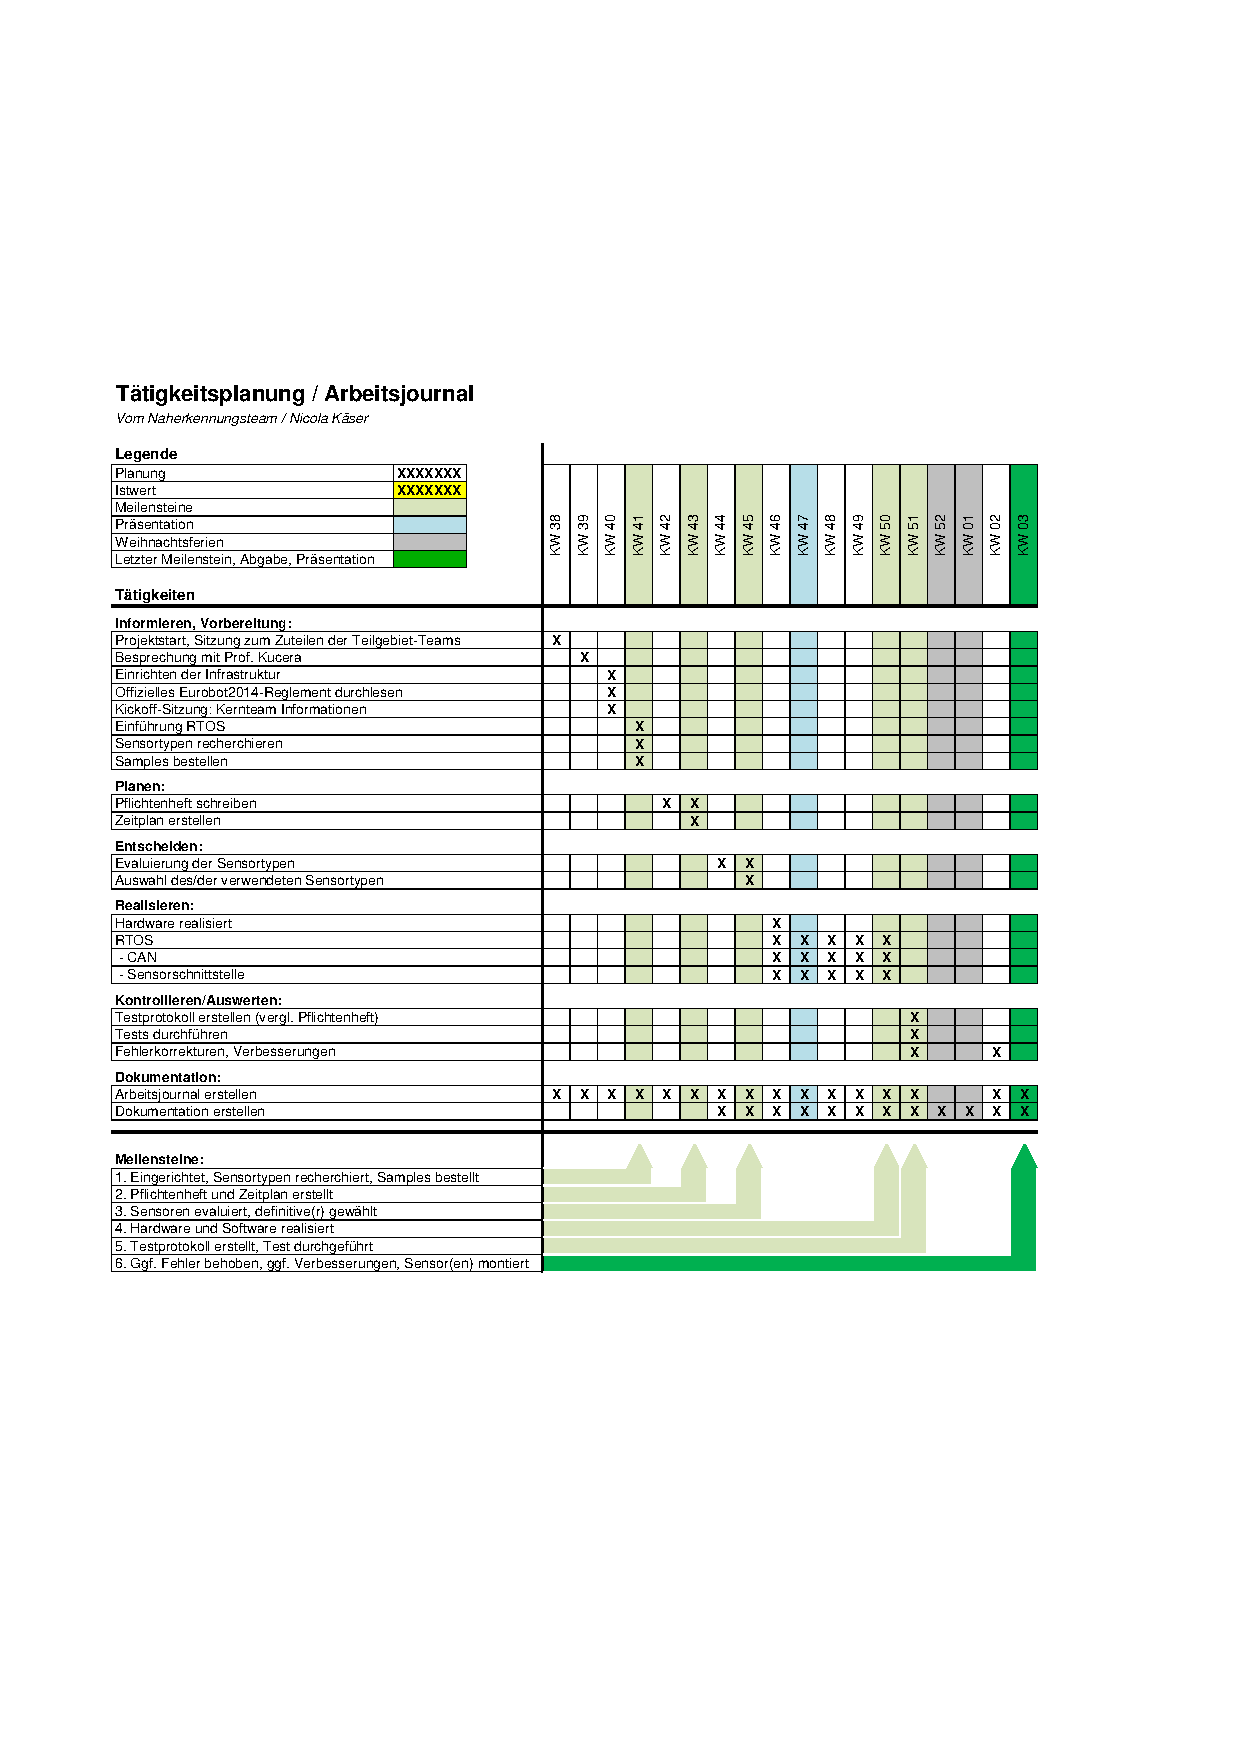
\includepdf[scale=1,page=-]{appendix/anhangA_Zeitplan.pdf} % Zeitplan
%%%%%%%%%%%%%%%%%%%%%%%%%%%%%%%%%%%%%%%%%%%%%%%%%%%%%%%%%%%%%%%%%%%%%%%%%%%%%%%
% Titel:   Anhang
% Autor:   Nicola K�ser
%%%%%%%%%%%%%%%%%%%%%%%%%%%%%%%%%%%%%%%%%%%%%%%%%%%%%%%%%%%%%%%%%%%%%%%%%%%%%%%
\chapter{Anhang B: Offizielles Reglement Eurobot 2014}\label{ch:anhang_b}
	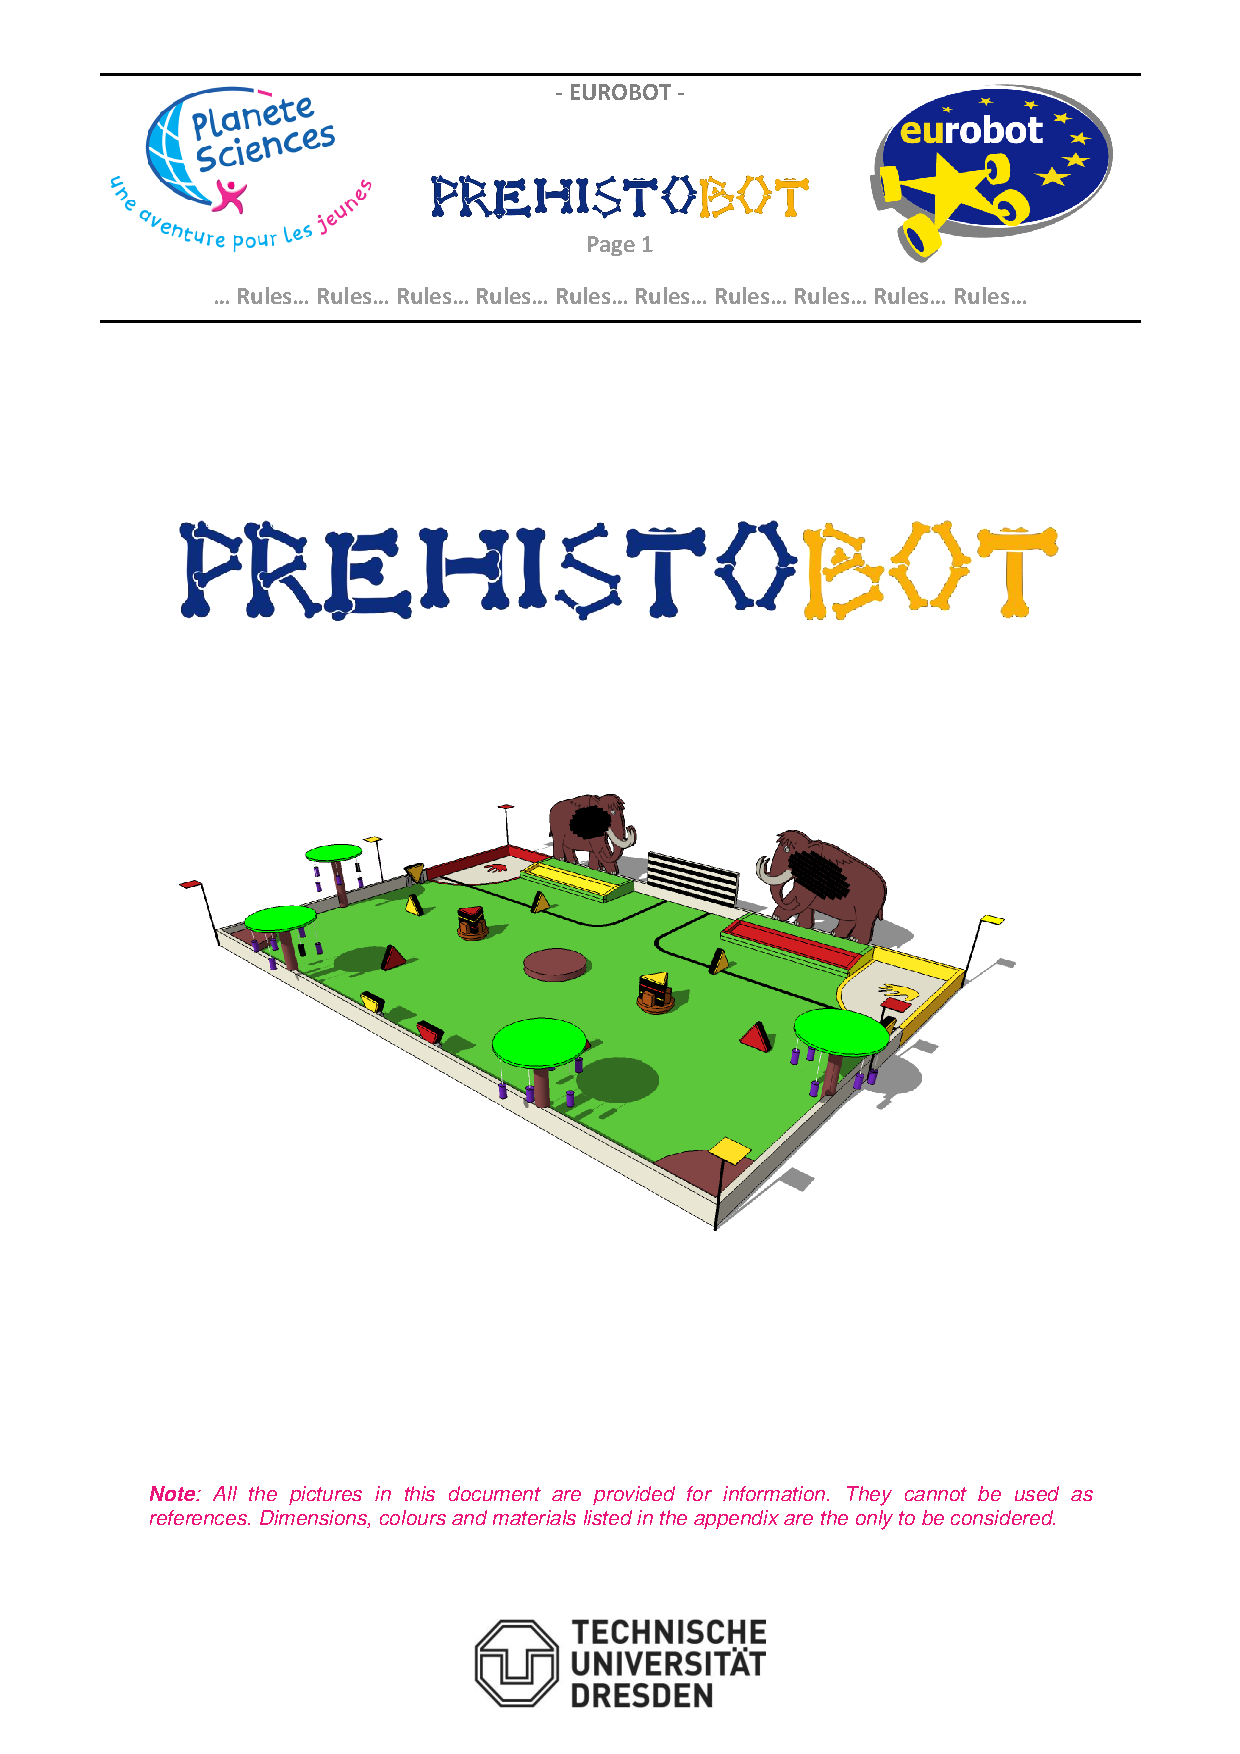
\includepdf[scale=1,pages=-]{appendix/anhangB_Reglement.pdf} % Reglement
%
%
%
%%%%%%%%%%%%%%%%%%%%%%%%%%%%%%%%%%%%%%%%%%%%%%%%%%%%%%%%%%%%%%%%%%%%%%%%%%%%%%%
% Stichwortverzeichnis
%%%%%%%%%%%%%%%%%%%%%%%%%%%%%%%%%%%%%%%%%%%%%%%%%%%%%%%%%%%%%%%%%%%%%%%%%%%%%%%
\renewcommand{\indexname}{Stichwortverzeichnis}
\printindex
%
%
%
\end{document}
